\documentclass[10pt, a4paper]{article}
\usepackage[paper=a4paper, left=1.5cm, right=1.5cm, bottom=1.5cm, top=2.5cm]{geometry}
\usepackage[utf8]{inputenc}
\usepackage[T1]{fontenc}
\usepackage[spanish]{babel}
\usepackage{indentfirst}
\usepackage{fancyhdr}
\usepackage{lastpage}
\usepackage{calc}
\usepackage{caratula}
\usepackage{marvosym} % para \Faxmachine !
\usepackage{graphicx}
\usepackage{float}
\usepackage{algpseudocode}
\usepackage{multicol}
\usepackage[hidelinks]{hyperref}
%\sloppy
\parskip=5pt % 10pt es el tamano de fuente

\usepackage{stringenc}
\usepackage{pdfescape}
\usepackage{listings}
\lstset{
	extendedchars=true,
    literate={á}{{\'a}}1 {é}{{\'e}}1 {í}{{\'i}}1 {ó}{{\'o}}1 {ú}{{\'u}}1 {ñ}{{\~n}}1,
    basicstyle=\ttfamily\small,
    tabsize=2,
    breaklines=true,
    breakatwhitespace=true,
}


\begin{document}
\title{PLP - TP1}
\materia{Paradigmas de Lenguajes de Programación}
\submateria{Primer cuatrimestre 2017}
\titulo{Trabajo Práctico 1\\Programación Funcional}
\subtitulo{Naves Espaciales}
\begin{center}
    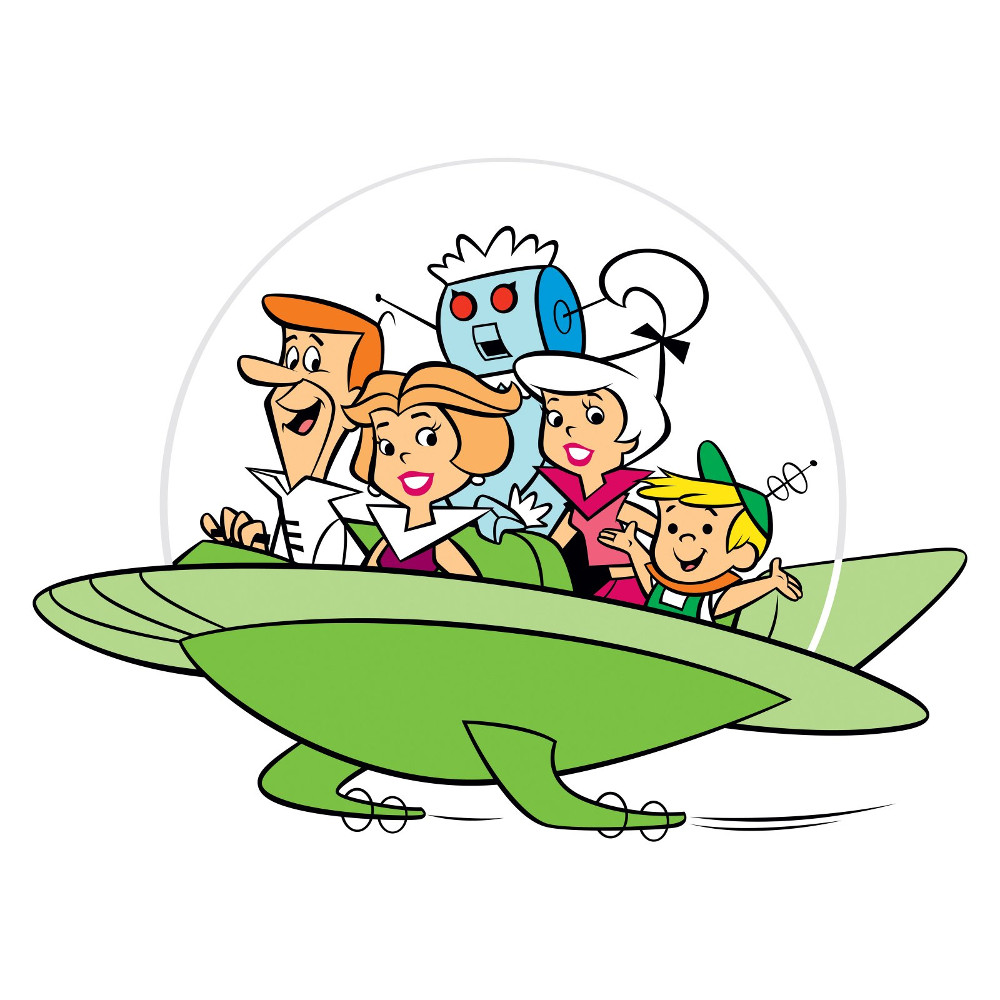
\includegraphics[width=0.6\textwidth]{spaceship.jpg}
\end{center}
\grupo{Grupo: Pescado Ravioloso}
\integrante{Alejandro González}{32/13}{gonzalezalejandro1592@gmail.com}
\integrante{Diego Sueiro}{75/90}{dsueiro@gmail.com}
\integrante{Malena Ivnisky}{421/12}{malenaivnisky@gmail.com}

\maketitle

\newpage

\section{Naves para pruebas}
\lstinputlisting[language=Haskell, firstline=9, lastline=36]{../Main.hs}

\section{Ejercicio 1}
\lstinputlisting[language=Haskell, firstline=25, lastline=35]{../NavesEspaciales.hs}

\section{Ejercicio 2}
\lstinputlisting[language=Haskell, firstline=38, lastline=48]{../NavesEspaciales.hs}
\subsection{Tests}
\lstinputlisting[language=Haskell, firstline=54, lastline=58]{../Main.hs}

\section{Ejercicio 3}
\lstinputlisting[language=Haskell, firstline=52, lastline=53]{../NavesEspaciales.hs}
\subsection{Tests}
\lstinputlisting[language=Haskell, firstline=62, lastline=64]{../Main.hs}

\section{Ejercicio 4}
\lstinputlisting[language=Haskell, firstline=57, lastline=61]{../NavesEspaciales.hs}
\subsection{Tests}
\lstinputlisting[language=Haskell, firstline=68, lastline=78]{../Main.hs}

\section{Ejercicio 5}
\lstinputlisting[language=Haskell, firstline=65, lastline=101]{../NavesEspaciales.hs}
\subsection{Tests}
\lstinputlisting[language=Haskell, firstline=82, lastline=95]{../Main.hs}

\section{Ejercicio 6}
\lstinputlisting[language=Haskell, firstline=104, lastline=105]{../NavesEspaciales.hs}
\subsection{Tests}
\lstinputlisting[language=Haskell, firstline=99, lastline=102]{../Main.hs}

\section{Ejercicio 7}
\lstinputlisting[language=Haskell, firstline=109, lastline=118]{../NavesEspaciales.hs}
\subsection{Tests}
\lstinputlisting[language=Haskell, firstline=106, lastline=108]{../Main.hs}

\section{Ejercicio 8}
\lstinputlisting[language=Haskell, firstline=121, lastline=141]{../NavesEspaciales.hs}
\subsection{Tests}
\lstinputlisting[language=Haskell, firstline=112, lastline=125]{../Main.hs}
\end{document}
